\documentclass[10pt,twocolumn,a4paper]{article}
\usepackage[margin=1.45cm,bottom=1.65cm,top=1.65cm]{geometry}
\usepackage{amsmath,amssymb}
\usepackage{graphicx}
\usepackage{booktabs}
\usepackage{hyperref}

\hypersetup{
    colorlinks=true,
    linkcolor=blue,
    citecolor=blue,
    urlcolor=blue
}

\renewcommand{\topfraction}{0.95}
\renewcommand{\bottomfraction}{0.95}
\renewcommand{\dbltopfraction}{0.95}
\renewcommand{\textfraction}{0.05}
\renewcommand{\floatpagefraction}{0.85}
\renewcommand{\dblfloatpagefraction}{0.85}

\setlength{\abovedisplayskip}{4pt}
\setlength{\belowdisplayskip}{4pt}
\setlength{\textfloatsep}{8pt plus 2pt minus 2pt}
\setlength{\dbltextfloatsep}{8pt plus 2pt minus 2pt}

\title{\textbf{When Harmonic ZNE Fails: Equal-Budget, Out-of-Family Noise, and Optimizer-Instability Audits on NISQ Devices}}

\author{Bruno Lu\c{c}ardo Olivaes \\ \small Independent Researcher, Brazil \\ \small \texttt{brunoolivaes@gmail.com} $\cdot$ ORCID: 0009-0003-5351-446X}

\date{November 2026 (v3.0 Equal-Budget \& Out-of-Family Audit)}

\begin{document}
\maketitle

\begin{abstract}
\noindent Zero-Noise Extrapolation (ZNE) is widely used on Noisy Intermediate-Scale Quantum (NISQ) processors, yet head-to-head comparisons frequently omit equal-shot-budget unmitigated baselines, out-of-family noise stress tests, and non-linear optimizer instability rates. Here we evaluate polynomial, exponential, forced damped harmonic, stability-gated automatic Lomb--Scargle (\texttt{Auto\_LombScargle\_ZNE}), and two-qubit Clifford Pauli-Twirled ZNE across four 1-qubit noise/schedule regimes (A1--A4, $K=25$ seeds, up to $N_{\mathrm{total}} = 32{,}768$ shots/seed) and an entangled 4-qubit Transverse-Field Ising Model (TFIM) Trotter circuit ($3$ steps, $18$ $\mathrm{CX}$ gates, $K=20$ seeds, $N_{\mathrm{total}} = 24{,}000$ shots/seed) in Qiskit 2.x (\texttt{AerSimulator}). In the in-family deep 1-qubit coherent Ramsey benchmark (A1, $s \le 17$), both forced Harmonic ZNE and stability-gated \texttt{Auto\_LombScargle\_ZNE} reduce Mean Absolute Error (MAE) to $0.0084 \pm 0.0012$ vs.\ $0.0482 \pm 0.0004$ for the equal-shot unmitigated baseline ($-82.6\%$, $z = +31.74\,\mathrm{SE}$, $0\%$ instability). Conversely, under out-of-family perturbations—short coherent scales (A2, $s \le 6$), monotonic amplitude damping plus depolarizing relaxation (A3), and bi-chromatic quasi-static Gaussian drift (A4)—forced Harmonic ZNE exhibits $100\%$ optimizer instability ($\mathrm{MAE} = 0.2007\text{--}0.3601$). In 4-qubit TFIM circuits, forced Harmonic ZNE collapses with $100\%$ instability at every coupling strength ($\mathrm{MAE} = 2.2868$ at $\epsilon = 0.04\,$rad vs.\ $0.1450 \pm 0.0008$ equal-budget unmitigated). Stability-gating (\texttt{unstable\_fit} combining covariance condition number $> 10^4$ and $2\%$ bound saturation) eliminates harmonic divergence ($0\%$ instability across A2--A4 and TFIM), while Pauli Twirling + ZNE reduces 4-qubit MAE by $75.2\%\text{--}81.3\%$ vs.\ the equal-budget unmitigated baseline—and maintains $86.8\%$ reduction ($0.0383 \pm 0.0070$ vs.\ $0.2911 \pm 0.0012$, $z = +35.55\,\mathrm{SE}$) even when single-qubit twirl frame gates (\texttt{x, y, z}) carry realistic depolarizing and coherent errors.
\end{abstract}

\section{Introduction}
Current quantum hardware operates in the Noisy Intermediate-Scale Quantum (NISQ) regime~\cite{preskill2018}, where gate errors reflect both stochastic decoherence and systematic coherent drift (residual Stark shifts, calibration detuning, and $ZZ$ crosstalk)~\cite{kandala2019,hashim2021}. Zero-Noise Extrapolation (ZNE)~\cite{temme2017,li2017,giurgica2020} estimates noiseless expectation values without ancilla qubits by running circuits across amplified noise scales $\lambda_j \ge 1$ and extrapolating to $\lambda \to 0$.

When coherent noise accumulates periodically with $\lambda$, low-order polynomials and pure exponentials can fail or invert sign. Spectral extensions based on the Lomb--Scargle periodogram~\cite{lomb1976,scargle1982} attempt to fit damped harmonic trajectories $E(\lambda) = E_0 e^{-\gamma \lambda}\cos(\omega \lambda + \phi)$, whereas Clifford Pauli Twirling~\cite{wallman2016,hashim2021} tailors coherent two-qubit errors into stochastic Pauli channels prior to ZNE.

Evaluating mitigation honestly requires three methodological controls often missing from proof-of-concept benchmarks: (1) an \textbf{equal-shot-budget unmitigated baseline} spending the entire shot budget $N_{\mathrm{total}}$ on $\lambda = 1$ alongside an equal-budget \textbf{twirl-only baseline} without extrapolation, plus explicit compiled-circuit count tracking ($1$ vs.\ $6$ vs.\ $12$ vs.\ $48$ circuits/seed); (2) \textbf{out-of-family noise channels and restricted scale horizons} outside the mono-mode sinusoidal ansatz; and (3) explicit \textbf{non-linear optimizer stability auditing} and finite Pauli-frame error robustness. Version 3.0 addresses all three requirements quantitatively.

\section{Methodology and Mitigation Architectures}

\subsection{Transmon Noise Models and Twirl Frame Errors}
All experiments run via Qiskit 2.x (\texttt{AerSimulator}). In 4-qubit TFIM circuits, single-qubit gates (\texttt{rx, rz, h}) experience $p_1 = 10^{-3}$ depolarizing noise and coherent $R_Z(0.5\epsilon)$ phase drift, while $\mathrm{CX}$ gates incur $p_2 = 1.2 \times 10^{-2}$ depolarizing error plus coherent $R_{ZZ}(\epsilon) \cdot (I \otimes R_Z(\epsilon))$. To test whether Pauli Twirling gains rely on noiseless frame insertions, we additionally evaluate a \textbf{noisy-twirl-frame} configuration at $\epsilon = 0.08\,$rad where inserted Pauli frame gates (\texttt{x, y, z}) carry depolarizing error $p_1 = 10^{-3}$ and coherent shift $R_Z(0.25\epsilon)$.

\subsection{Fractional Folding, Clifford Twirling, and Budget Accounting}
Non-uniform fractional unitary folding~\cite{giurgica2020} scales $\mathrm{CX}$ vs.\ 1-qubit gates at a $10:1$ weight behind compiler barriers while preserving $U_{\mathrm{folded}} = U$, yielding $\lambda \in \{1.000, 1.398, 1.796, 2.294, 2.851, 3.498\}$ on 4-qubit TFIM. Every seed enforces a matched shot ceiling ($N_{\mathrm{total}} = 24{,}000$ in 4Q TFIM; $32{,}768$ in 8-scale 1Q; $24{,}576$ in 6-scale 1Q):
\begin{itemize}
    \item \texttt{Unmitigated\_Equal\_Budget}: $1$ circuit ($\lambda=1$) $\times N_{\mathrm{total}}$ shots.
    \item \texttt{Pauli\_Twirl\_Only\_Equal\_Budget}: $12$ twirled circuits ($\lambda=1$) $\times 2{,}000 = 24{,}000$ shots.
    \item Untwirled ZNE (Quadratic / Exp / Harmonic / Auto): $6$ scaled circuits $\times 4{,}000 = 24{,}000$ shots (Local Linear uses the first $4$ scales, $16{,}000$ shots).
    \item Pauli-Twirled ZNE (\texttt{Pauli\_Twirl\_Linear/Exp}): $4$ scales $\times 12$ twirls $= 48$ circuits $\times 500 = 24{,}000$ shots.
\end{itemize}

\subsection{Stability-Gated Lomb--Scargle Extrapolator}
The 4-parameter model $E(\lambda) = E_0 e^{-\gamma \lambda}\cos(\omega \lambda + \phi)$ fits bounded \texttt{curve\_fit} parameters $E_0 \in [-2,2]$, $\gamma \in [0, 1.5]$, $\omega \in [0.01, 3.0]$, $\phi \in [-0.35, 0.35]$. Because Scargle's asymptotic exponential False-Alarm Probability has a hard small-$N$ floor ($\mathrm{FAP} \ge 0.137$ at $N=8$), \texttt{Auto\_LombScargle\_ZNE} triggers harmonic candidate fitting when $\mathrm{FAP} < 0.05$ or ($N \le 12$ and explained variance $R^2_{\mathrm{peak}} = 2 z_{\max}/N \ge 0.60$), and \textbf{accepts} the harmonic fit if and only if \texttt{unstable\_fit} is \texttt{False}:
\begin{equation}
\texttt{unstable\_fit} \;\equiv\; \texttt{at\_bounds} \;\lor\; \big(\kappa(C_{\mathrm{cov}}) > 10^4\big) \;\lor\; \neg\mathrm{isfinite}(\kappa),
\end{equation}
where $\kappa(C_{\mathrm{cov}})$ is the covariance condition number and \texttt{at\_bounds} flags upper bounds within $2\%$ of span, non-zero lower bounds within $2\%$, or $\gamma \le 10^{-4}$. Unstable harmonic candidates automatically fall back to \texttt{Local\_Linear\_ZNE}.

\begin{table*}[t]
\centering
\caption{\textbf{Regime A (1-Qubit Echo, $K=25$ Seeds, $E_{\mathrm{ideal}}=+1.0000$): Out-of-Family Stress Tests and Equal-Budget Baselines.} Values show $\mathrm{MAE} \pm \mathrm{SE}$; parenthetical percentages indicate optimizer instability rates (\texttt{inst}) or automatic harmonic selection rate (\texttt{sel}) for \texttt{Auto\_LombScargle\_ZNE}.}
\label{tab:regime_a_audit}
\resizebox{\textwidth}{!}{%
\begin{tabular}{lcccc}
\toprule
\textbf{Method} & \textbf{A1: Deep Mono-Mode} & \textbf{A2: Short Coherent} & \textbf{A3: Amp.\ Damp + Depol} & \textbf{A4: Bi-Chromatic + $1/f$} \\
 & ($s\in\{1..17\}$, $32{,}768$ shots) & ($s\in\{1..6\}$, $24{,}576$ shots) & ($\theta=0$, $\gamma_{\mathrm{AD}}=0.015$) & ($\theta\in\{0.22,0.53\}$, $\sigma_\theta=0.07$) \\
\midrule
Unmitigated (1 scale, $4{,}096$ shots) & $0.0491 \pm 0.0011$ & $0.0496 \pm 0.0009$ & $0.0318 \pm 0.0007$ & $0.0892 \pm 0.0014$ \\
\textbf{Unmitigated Equal Budget} ($1$ circ.) & $0.0482 \pm 0.0004$ & $0.0487 \pm 0.0004$ & $0.0324 \pm 0.0002$ & $0.0904 \pm 0.0009$ \\
Global Quadratic ZNE & $0.3199 \pm 0.0011$ & $\mathbf{0.0349 \pm 0.0030}$ & $0.0046 \pm 0.0006$ & $\mathbf{0.0387 \pm 0.0062}$ \\
Local Linear ZNE ($4$ circ.) & $0.1197 \pm 0.0018$ & $0.0947 \pm 0.0018$ & $0.0044 \pm 0.0006$ & $0.1667 \pm 0.0041$ \\
Exponential ZNE & $0.5766 \pm 0.0014$ ($0\%$) & $0.2758 \pm 0.0026$ ($0\%$) & $\mathbf{0.0037 \pm 0.0004}$ ($0\%$) & $0.6979 \pm 0.0063$ ($0\%$) \\
\midrule
\textbf{Damped Harmonic ZNE (Forced)} & $\mathbf{0.0084 \pm 0.0012}$ ($0\%$ inst) & $0.3601 \pm 0.1899$ ($100\%$ inst) & $0.2956 \pm 0.1612$ ($100\%$ inst) & $0.2007 \pm 0.0129$ ($100\%$ inst) \\
\textbf{Auto Lomb--Scargle ZNE} & $\mathbf{0.0084 \pm 0.0012}$ ($100\%$ sel) & $0.0947 \pm 0.0018$ ($0\%$ sel) & $0.0044 \pm 0.0006$ ($0\%$ sel) & $0.1667 \pm 0.0041$ ($0\%$ sel) \\
\midrule
\textbf{Auto vs.\ Equal-Budget Unmit.} & $\mathbf{-82.6\%}$ ($z=+31.74\,\mathrm{SE}$) & $-94.5\%$ worse ($z=-24.58$) & $\mathbf{-86.4\%}$ ($z=+40.47\,\mathrm{SE}$) & $-84.4\%$ worse ($z=-17.97$) \\
\bottomrule
\end{tabular}%
}
\end{table*}

\begin{table*}[t]
\centering
\caption{\textbf{Regime B (4-Qubit TFIM Trotter, $\langle Z_0 \rangle_{\mathrm{ideal}} = -0.4081$, $K=20$ Seeds, $N_{\mathrm{total}} = 24{,}000$ Shots/Seed).} Compares equal-budget unmitigated and twirl-only baselines under ideal Pauli frames ($\epsilon \in \{0.00..0.14\}$) and noisy Pauli frames (\texttt{x,y,z} with $p_1=0.001$, $R_Z(0.25\epsilon)$ at $\epsilon=0.08$). Instability rates appear in brackets when non-zero.}
\label{tab:zne_benchmark}
\resizebox{\textwidth}{!}{%
\begin{tabular}{lcccc|c}
\toprule
\textbf{Method} \textit{(Circuits / Shots)} & $\epsilon = 0.00\,$rad & $\epsilon = 0.04\,$rad & $\epsilon = 0.08\,$rad & $\epsilon = 0.14\,$rad & $\epsilon = 0.08$ \textbf{(Noisy Frames)} \\
\midrule
Unmitigated ($1$ circ., $4\mathrm{k}$) & $0.0273 \pm 0.0027$ & $0.1484 \pm 0.0027$ & $0.2872 \pm 0.0032$ & $0.5347 \pm 0.0028$ & $0.2848 \pm 0.0026$ \\
\textbf{Unmitigated Equal Budget} ($1$ / $24\mathrm{k}$) & $0.0265 \pm 0.0014$ & $0.1450 \pm 0.0008$ & $0.2883 \pm 0.0017$ & $0.5322 \pm 0.0011$ & $0.2911 \pm 0.0012$ \\
\textbf{Pauli Twirl Only Eq.\ Budget} ($12$ / $24\mathrm{k}$) & $0.0259 \pm 0.0013$ & $0.0565 \pm 0.0037$ & $0.0991 \pm 0.0045$ & $0.1554 \pm 0.0084$ & $0.1167 \pm 0.0065$ \\
Local Linear ZNE ($4$ / $16\mathrm{k}$) & $0.0194 \pm 0.0036$ & $0.0407 \pm 0.0051$ & $0.0735 \pm 0.0056$ & $0.1002 \pm 0.0056$ & $0.0817 \pm 0.0063$ \\
Quadratic Richardson ZNE ($6$ / $24\mathrm{k}$) & $0.0396 \pm 0.0076$ & $0.1027 \pm 0.0089$ & $0.2086 \pm 0.0101$ & $0.2006 \pm 0.0086$ & $0.2370 \pm 0.0086$ \\
Exponential ZNE ($6$ / $24\mathrm{k}$) & $\mathbf{0.0156 \pm 0.0027}$ & $0.3763 \pm 0.0157$ & $0.5405 \pm 0.0017$ [1.0] & $0.7876 \pm 0.0012$ [1.0] & $0.5413 \pm 0.0013$ [1.0] \\
\midrule
\textbf{Pauli Twirl + Linear ZNE} ($48$ / $24\mathrm{k}$) & $0.0243 \pm 0.0035$ & $\mathbf{0.0347 \pm 0.0042}$ & $0.0766 \pm 0.0105$ & $0.1212 \pm 0.0158$ & $\mathbf{0.0383 \pm 0.0070}$ \\
\textbf{Pauli Twirl + Exp ZNE} ($48$ / $24\mathrm{k}$) & $0.0307 \pm 0.0047$ & $0.0363 \pm 0.0044$ & $\mathbf{0.0714 \pm 0.0082}$ [0.25] & $\mathbf{0.0997 \pm 0.0136}$ [0.20] & $0.0406 \pm 0.0069$ \\
\midrule
\textbf{Damped Harmonic ZNE} ($6$ / $24\mathrm{k}$) & $1.2701 \pm 0.1530$ [1.0] & $2.2868 \pm 0.0000$ [1.0] & $0.3042 \pm 0.0650$ [1.0] & $0.5550 \pm 0.0018$ [1.0] & $0.2493 \pm 0.0628$ [1.0] \\
\textbf{Auto Lomb--Scargle ZNE} ($6$ / $24\mathrm{k}$) & $0.0194 \pm 0.0036$ & $0.0407 \pm 0.0051$ & $0.0735 \pm 0.0056$ & $0.1002 \pm 0.0056$ & $0.0817 \pm 0.0063$ \\
\midrule
\textbf{Harmonic 2-SE Niche Confirmed?} & False ($z=-8.20$) & False ($z=-531.4$) & False ($z=-3.55$) & False ($z=-33.25$) & False ($z=-3.34$) \\
\textbf{Best Gain vs.\ Eq.\ Budget Unmit.} & $-41.1\%$ (Exp) & $\mathbf{-76.1\%}$ (Tw+Lin) & $\mathbf{-75.2\%}$ (Tw+Exp) & $\mathbf{-81.3\%}$ (Tw+Exp) & $\mathbf{-86.8\%}$ (Tw+Lin) \\
\bottomrule
\end{tabular}%
}
\end{table*}

\section{Benchmark Results}

\subsection{Regime A: In-Family Niche vs.\ Out-of-Family Breakdown}
Table~\ref{tab:regime_a_audit} demonstrates both the genuine single-mode niche and its fragility outside that family:
\begin{itemize}
    \item \textbf{A1 (In-Family Deep Mono-Mode):} \texttt{Auto\_LombScargle\_ZNE} selects the harmonic model on $100\%$ of seeds with $0\%$ instability, lowering MAE from $0.0482 \pm 0.0004$ (\texttt{Unmitigated\_Equal\_Budget}) to $0.0084 \pm 0.0012$ ($-82.6\%$, $z = +31.74\,\mathrm{SE}$).
    \item \textbf{A2--A4 (Short Scales, Monotonic Relaxation, and Bi-Chromatic $1/f$ Drift):} Forced Harmonic ZNE suffers $100\%$ optimizer instability across all three regimes ($\mathrm{MAE} = 0.3601$ in A2, $0.2956$ in A3, $0.2007$ in A4). The stability gate prevents catastrophic divergence ($0\%$ instability, $0\%$ harmonic selection) by falling back to local linear extrapolation. While this matches monotonic ZNE performance in A3 ($\mathrm{MAE} = 0.0044 \pm 0.0006$ vs.\ Exponential $0.0037$, $z = +40.47\,\mathrm{SE}$ over equal-budget unmitigated), local linear fallback itself loses to \texttt{Unmitigated\_Equal\_Budget} when noise trajectories bend within the first 4 scales without reaching an asymptotic tail (A2: $0.0947$ vs.\ $0.0487$; A4: $0.1667$ vs.\ $0.0904$). No mitigation beats quadratic or unmitigated on turned/beating A2/A4 trajectories uniformly via simple linear fitting.
\end{itemize}

\begin{figure*}[t]
\centering
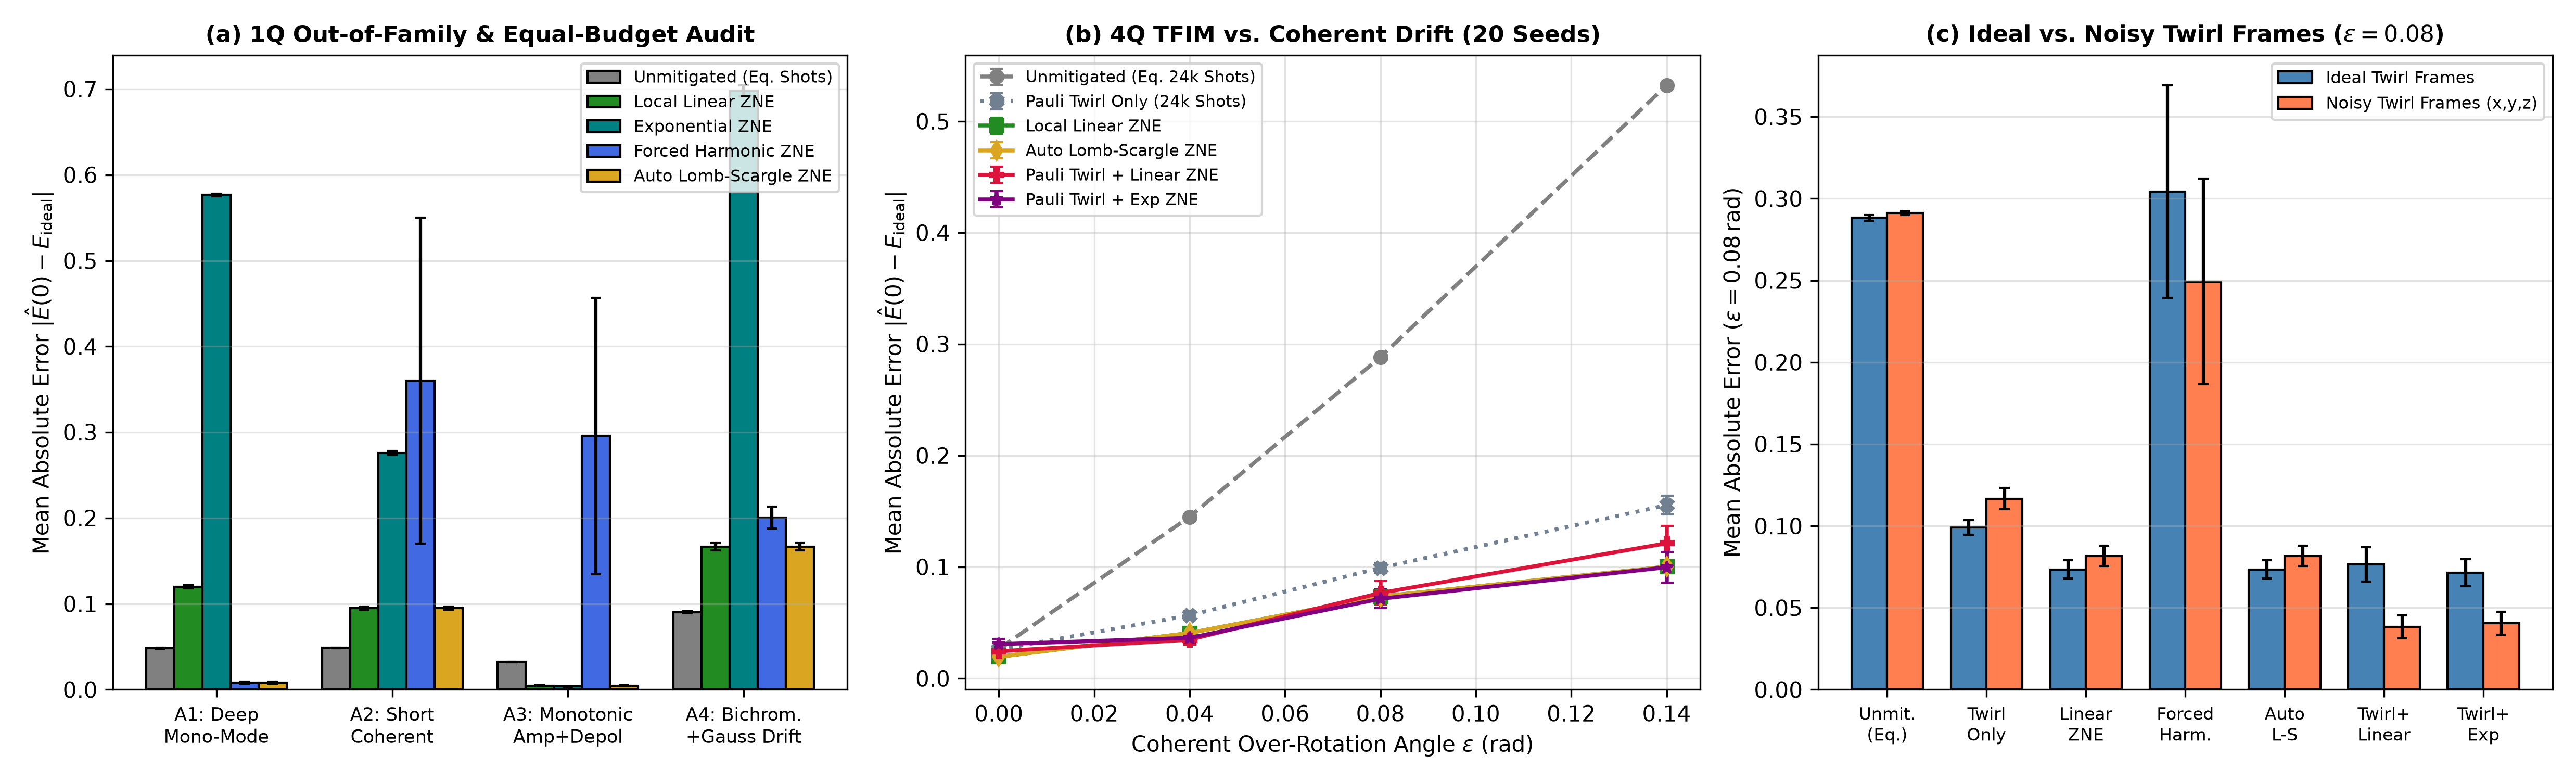
\includegraphics[width=\textwidth]{fig_fair_zne_comparison.png}
\caption{\textbf{Equal-budget, out-of-family, and noisy-frame QEM audit.} (a) 1-qubit Regime A1--A4 stress test showing Forced Harmonic ZNE breaking down ($100\%$ instability) in A2--A4 while \texttt{Auto\_LombScargle\_ZNE} isolates A1 ($0.0084$) and safely avoids divergence. (b) 4-qubit TFIM MAE vs.\ coherent angle $\epsilon$ comparing \texttt{Unmitigated\_Equal\_Budget}, \texttt{Pauli\_Twirl\_Only\_Equal\_Budget}, \texttt{Auto\_LombScargle\_ZNE}, and Pauli-Twirled ZNE. (c) Ideal vs.\ noisy Pauli twirl frame (\texttt{x, y, z}) comparison at $\epsilon = 0.08\,$rad.}
\label{fig:benchmark_results}
\end{figure*}

\subsection{Regime B: 4-Qubit TFIM, Equal-Budget Baselines, and Noisy Twirl Frames}
Table~\ref{tab:zne_benchmark} and Figure~\ref{fig:benchmark_results} isolate what drives error reduction in multi-qubit entangled circuits:
\begin{enumerate}
    \item \textbf{Harmonic ZNE Divergence and Stability Gate Recovery:} Forced Harmonic ZNE triggers $100\%$ instability at all five 4Q TFIM settings ($\mathrm{MAE} = 1.2701$ at $\epsilon=0$, $2.2868$ at $\epsilon=0.04$), whereas \texttt{Auto\_LombScargle\_ZNE} maintains $0\%$ instability by falling back cleanly to local linear ZNE ($0.0194\text{--}0.1002$).
    \item \textbf{Twirling Only vs.\ Twirling + ZNE vs.\ Equal-Budget Unmitigated:} Merely executing Pauli Twirling at $\lambda=1$ without extrapolation (\texttt{Pauli\_Twirl\_Only\_Equal\_Budget}, $12$ circuits) already cuts $\epsilon=0.08$ error from $0.2883$ to $0.0991$ ($-65.6\%$). Adding ZNE across $4$ scales ($48$ circuits) further lowers error to $0.0714 \pm 0.0082$ ($-75.2\%$ vs.\ equal-budget unmitigated, $z = +25.89\,\mathrm{SE}$), though at high $\epsilon = 0.14\,$rad untwirled \texttt{Linear\_ZNE} ($0.1002$) performs comparably to \texttt{Pauli\_Twirl\_Exp\_ZNE} ($0.0997$, which shows $20\%$ exponential fit instability).
    \item \textbf{Robustness to Finite Twirl Frame Gate Errors:} Adding realistic depolarizing and coherent errors directly to inserted \texttt{x, y, z} twirl gates at $\epsilon = 0.08\,$rad leaves \texttt{Pauli\_Twirl\_Linear\_ZNE} at $\mathrm{MAE} = 0.0383 \pm 0.0070$ ($-86.8\%$ vs.\ equal-budget unmitigated $0.2911 \pm 0.0012$, $z = +35.55\,\mathrm{SE}$, $0\%$ instability), confirming that Pauli Twirling remains advantageous even without ideal zero-error frame gates.
\end{enumerate}

\section{Discussion and Operational Conclusions}
Our audit demonstrates that Harmonic ZNE does \emph{not} provide a general-purpose NISQ advantage: its $82.6\%$ MAE reduction (vs.\ equal-budget unmitigated) is strictly confined to well-sampled, single-mode coherent drift (A1). On short scales (A2), monotonic relaxation (A3), bi-chromatic $1/f$ drift (A4), and multi-qubit non-commuting TFIM circuits, forced 4-parameter harmonic fitting hits parameter bounds and diverges with $100\%$ instability. Adding explicit covariance-conditioning and bound-saturation gates (\texttt{Auto\_LombScargle\_ZNE}) eliminates divergence safely, while Clifford Pauli Twirling combined with low-order ZNE provides substantial reductions ($75.2\%\text{--}86.8\%$) over equal-shot unmitigated and twirl-only baselines—at an explicit compilation cost of $48$ circuit variants per seed versus $1$ unmitigated or $12$ twirl-only circuits.

\section*{Code and Data Availability}
Code, CI tests ($7/7$ \texttt{pytest}), JSON audit tables, and manuscript sources are archived under Zenodo DOI \href{https://doi.org/10.5281/zenodo.24121693}{\texttt{10.5281/zenodo.24121693}} (\url{https://github.com/bruno-olivaes/qiskit-lombscargle-zne}).

\begin{thebibliography}{99}
\footnotesize
\setlength{\itemsep}{0pt}
\setlength{\parskip}{0pt}
\bibitem{preskill2018}
J. Preskill, Quantum \textbf{2}, 79 (2018).
\bibitem{temme2017}
K. Temme, S. Bravyi, and J. M. Gambetta, Phys. Rev. Lett. \textbf{119}, 180509 (2017).
\bibitem{li2017}
Y. Li and S. C. Benjamin, Phys. Rev. X \textbf{7}, 021050 (2017).
\bibitem{giurgica2020}
T. Giurgica-Tiron, Y. Hindy, R. LaRose, A. Mari, and W. J. Zeng, in \textit{2020 IEEE QCE} (IEEE, 2020), pp. 306--316.
\bibitem{kandala2019}
A. Kandala et al., Nature \textbf{567}, 491 (2019).
\bibitem{wallman2016}
J. J. Wallman and J. Emerson, Phys. Rev. A \textbf{94}, 052325 (2016).
\bibitem{hashim2021}
A. Hashim et al., Phys. Rev. X \textbf{11}, 041039 (2021).
\bibitem{lomb1976}
N. R. Lomb, Astrophys. Space Sci. \textbf{39}, 447 (1976).
\bibitem{scargle1982}
J. D. Scargle, Astrophys. J. \textbf{263}, 835 (1982).
\end{thebibliography}

\end{document}
